\documentclass[10pt]{article}
\usepackage[polish]{babel}
\usepackage[utf8]{inputenc}
\usepackage[T1]{fontenc}
\usepackage{amsmath}
\usepackage{amsfonts}
\usepackage{amssymb}
\usepackage[version=4]{mhchem}
\usepackage{stmaryrd}
\usepackage{bbold}
\usepackage{graphicx}
\usepackage[export]{adjustbox}
\graphicspath{ {./images/} }
\usepackage{hyperref}
\hypersetup{colorlinks=true, linkcolor=blue, filecolor=magenta, urlcolor=cyan,}
\urlstyle{same}

\title{Metody Obliczeniowe w Nauce i Technice }


\author{Maciej Grzybacz}
\date{}


\begin{document}
\maketitle
05.05 .2024

\section*{Treści zadan}
\begin{enumerate}
  \item Napisz program, który:
\end{enumerate}

(a) Jako parametr pobiera rozmiar układu równań $n$ i ilość rozwiązań $b \in \mathbb{R}^{n}$.

(b) Generuje macierz układu $A \in \mathbb{R}^{n \times n}$ i wektor wyrazów wolnych $b \in$ $\mathbb{R}^{n}$

(c) Rozwiązuje układ równań $A x=b$ na trzy sposoby:

i. przez dekompozycję LU macierzy $A: A=L U$;

ii. przez odwrócenie macierzy $A$ : $x=A^{-1} b$ i sprawdzić czy $A A^{-1}=$ $I$ oraz $A^{-1} A=I$ (macierz jednostkowa);

iii. przez dekompozycję QR macierzy $A: A=Q R$.

(d) Sprawdzić poprawność rozwiązania (tj., czy $A x=b$ ).

(e) Zmierzyć całkowity czas rozwiązania układu.

(f) Porównać czasy z trzech sposobów: przez dekompozycję LU, przez odwrócenie macierzy i przez dekompozycję QR.

\begin{enumerate}
  \setcounter{enumi}{1}
  \item Zadanie domowe: Narysuj wykres zależności całkowitego czasu rozwiązania układu (LU, QR, odwrócenie macierzy) od rozmiaru układu równań. Wykonaj pomiary dla 5 wartości $n$ z przedziału od 10 do 100 . Uwaga: można się posłużyć funkcjami z biblioteki numerycznej danego języka programowania.
\end{enumerate}

\section*{Zadanie 1A}
Program napisany w Pythonie generuje losową macierz układu $A \in \mathbb{R}^{n \times n}$ oraz wektor wyrazów wolnych $b \in \mathbb{R}^{n}$. Następnie rozwiązuje układ równań $A x=b$ za pomocą dekompozycji LU.

Dekompozycja LU dzieli macierz $A$ na iloczyn dwóch macierzy trójkątnych: dolnej (L) i górnej (U). Rozwiązanie uzyskuje się poprzez rozwiązanie dwóch układów równań:

$$
\begin{aligned}
L y & =b \\
U x & =y
\end{aligned}
$$

Program używa funkcji lu\_factor i lu\_solve z biblioteki scipy.linalg.

\subsection*{Kod programu w Pythonie}
\begin{verbatim}
import numpy as np
from scipy.linalg import lu, lu_solve, lu_factor
def solve_with_lu(n):
    # Generowanie losowej macierzy A i wektora b
    A = np.random.randn(n, n)
    b = np.random.randn(n)
    # Dekompozycja LU
    lu_piv = lu_factor(A)
    x = lu_solve(lu_piv, b)
    return A, b, x
\end{verbatim}

Listing 1: Rozwiązywanie układu równań za pomocą dekompozycji LU

\section*{Zadanie 1B}
Program napisany w Pythonie generuje losową macierz układu $A \in \mathbb{R}^{n \times n}$ oraz wektor wyrazów wolnych $b \in \mathbb{R}^{n}$. Następnie rozwiązuje układ równań $A x=b$ poprzez odwrócenie macierzy.

Rozwiązanie układu równań uzyskuje się poprzez obliczenie odwrotności macierzy $A$ oraz pomnożenie jej przez wektor $b$ :

$$
x=A^{-1} b
$$

Program sprawdza również, czy $A A^{-1}=I$ oraz $A^{-1} A=I$, gdzie $I$ jest macierzą jednostkowa.

\subsection*{Kod programu w Pythonie}
\begin{verbatim}
import numpy as np
def solve_with_inverse(n):
    # Generowanie losowej macierzy A i wektora b
    A = np.random.randn(n, n)
    b = np.random.randn(n)
    # Odwracanie macierzy A
    A_inv = np.linalg.inv(A)
    x = np.dot(A_inv, b)
    # Sprawdzenie czy A * A_inv = I i A_inv * A = I
    identity_1 = np.allclose(np.dot(A, A_inv), np.eye(n))
    identity_2 = np.allclose(np.dot(A_inv, A), np.eye(n))
    return A, b, x, identity_1, identity_2
\end{verbatim}

Listing 2: Rozwiązywanie układu równań poprzez odwrócenie macierzy

\section*{Zadanie 1C}
Program napisany w Pythonie generuje losową macierz układu $A \in \mathbb{R}^{n \times n}$ oraz wektor wyrazów wolnych $b \in \mathbb{R}^{n}$. Następnie rozwiązuje układ równań $A x=b$ poprzez dekompozycję QR.

Dekompozycja QR dzieli macierz $A$ na iloczyn ortogonalnej macierzy $Q$ oraz trójkątnej macierzy $R$ :

$$
A=Q R
$$

Rozwiązanie uzyskuje się poprzez rozwiązanie układu równań:

$$
R x=Q^{T} b
$$

Program używa funkcji qr i solve\_triangular z biblioteki scipy.linalg.

\subsection*{Kod programu w Pythonie}
\begin{verbatim}
import numpy as np
from scipy.linalg import qr, solve_triangular
def solve_with_qr(n):
    # Generowanie losowej macierzy A i wektora b
    A = np.random.randn(n, n)
    b = np.random.randn(n)
    # Dekompozycja QR
    Q, R = qr(A)
    x = solve_triangular(R, np.dot(Q.T, b))
    return A, b, x, Q, R
\end{verbatim}

Listing 3: Rozwiązywanie układu równań poprzez dekompozycję QR

\section*{Weryfikacja poprawności}
Aby sprawdzić poprawność rozwiązania układu równań $A x=b$, obliczamy iloczyn $A x$ i porównujemy go z wektorem $b$. Jeśli $A x \approx b$ (z dopuszczalnym błędem numerycznym), rozwiązanie uważa się za poprawne. Dla metody odwrócenia macierzy dodatkowo weryfikujemy, czy macierz odwrotna spełnia właściwości macierzy jednostkowej: $A A^{-1}=I$ i $A^{-1} A=I$. W przypadku dekompozycji LU oraz QR sprawdzamy poprawność, obliczając odpowiednio iloczyn $L U$ oraz $Q R$ i porównujac je z oryginalną macierzą $A$. W każdym przypadku wykorzystujemy funkcję np.allclose, aby uwzględnić błędy numeryczne.

\section*{Pomiary czasu wykonania}
Aby ocenić efektywność różnych metod rozwiązywania układów równań $A x=b$, zmierzyłem czas wykonania dla trzech metod:

\begin{enumerate}
  \item Dekompozycja LU,

  \item Odwrócenie macierzy $A$,

  \item Dekompozycja QR.

\end{enumerate}

Testy zostały przeprowadzone dla macierzy o rozmiarach od 10 do $100 \mathrm{z}$ krokiem 10. Każda metoda była testowana na losowo wygenerowanych macierzach układu $A$ i wektorach $b$. Wyniki przedstawiono w tabeli 1.

\begin{center}
\begin{tabular}{|c|c|c|c|}
\hline
Rozmiar & Czas LU (s) & Czas Inverse (s) & Czas QR (s) \\
\hline
10 & 0.000053 & 0.000038 & 0.000086 \\
20 & 0.000129 & 0.000131 & 0.000182 \\
30 & 0.000226 & 0.000207 & 0.000325 \\
40 & 0.000457 & 0.000353 & 0.000613 \\
50 & 0.000683 & 0.000616 & 0.000864 \\
60 & 0.001011 & 0.000817 & 0.001194 \\
70 & 0.001406 & 0.001084 & 0.001621 \\
80 & 0.001929 & 0.001412 & 0.002198 \\
90 & 0.002453 & 0.001725 & 0.002851 \\
100 & 0.003076 & 0.002125 & 0.003647 \\
\hline
\end{tabular}
\end{center}

Tabela 1: Porównanie czasu rozwiązywania układu równań dla różnych metod rozwiązania układu

\begin{center}
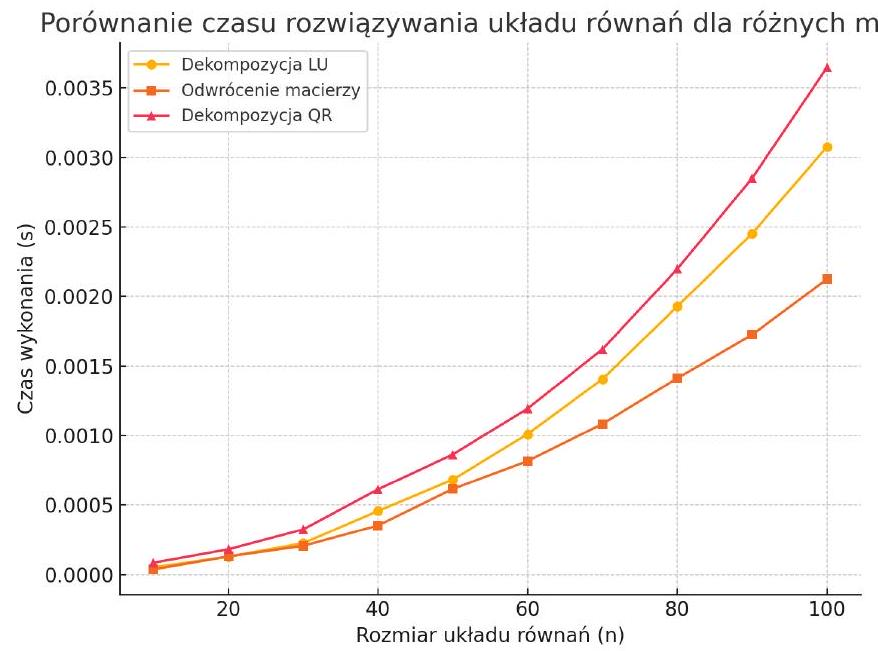
\includegraphics[max width=\textwidth]{2024_05_12_58df1b62820eb2f3d9ceg-5}
\end{center}

\section*{Wnioski}
Na podstawie wykresu można wyciągnąć następujące wnioski:

\begin{itemize}
  \item Dekompozycja LU okazuje się być szybsza od innych metod dla mniejszych rozmiarów macierzy,
  \item Metoda odwrócenia macierzy $A$ ma umiarkowany czas wykonania, ale jej efektywność spada dla większych rozmiarów macierzy,
  \item Dekompozycja QR wykazuje się większą stabilnością numerycznac, ale jej czas wykonania jest nieco dłuższy w porównaniu z dekompozycją LU.
\end{itemize}

\section*{1 Bibliografia}
\begin{itemize}
  \item Włodzimierz Funika Materialy ze strony internetowej
  \item Katarzyna Rycerz Wyklad z przedmiotu Metody Obliczeniowe w Nauce $i$ Technice
  \item \href{https://www.wolframalpha.com}{https://www.wolframalpha.com}
  \item \href{https://pl.wikipedia.org/wiki/Rozklad_QR}{https://pl.wikipedia.org/wiki/Rozklad\_QR}
  \item \href{https://pl.wikipedia.org/wiki/Macierz_odwrotna}{https://pl.wikipedia.org/wiki/Macierz\_odwrotna}
  \item \href{https://pl.wikipedia.org/wiki/Metoda_LU}{https://pl.wikipedia.org/wiki/Metoda\_LU}
\end{itemize}

\end{document}